% Shared preamble for the Generative AI (CS 782/882, Fall 2026) lecture notes.
% Each weekNN-notes.tex file inlines this block so it compiles on its own.
\documentclass[11pt]{article}
\usepackage[margin=1in]{geometry}
\usepackage[T1]{fontenc}
\usepackage[utf8]{inputenc}
\usepackage{lmodern}
\usepackage{amsmath,amssymb,amsthm,mathtools,bm}
\usepackage{enumitem}
\usepackage{graphicx}
\usepackage{booktabs}
\usepackage{xcolor}
\usepackage{tikz}
\usetikzlibrary{arrows.meta,positioning,calc,shapes}
\usepackage{listings}
\usepackage[colorlinks=true,linkcolor=blue!60!black,urlcolor=blue!60!black,citecolor=blue!60!black]{hyperref}

\newcommand{\E}{\mathbb{E}}
\newcommand{\Var}{\mathrm{Var}}
\newcommand{\KL}{\mathrm{KL}}
\newcommand{\given}{\,\vert\,}
\newcommand{\R}{\mathbb{R}}
\DeclareMathOperator*{\argmax}{arg\,max}
\DeclareMathOperator*{\argmin}{arg\,min}
\newtheorem{theorem}{Theorem}
\newtheorem{lemma}{Lemma}
\newtheorem{definition}{Definition}
\theoremstyle{remark}
\newtheorem*{remark}{Remark}

\lstset{basicstyle=\ttfamily\small,breaklines=true,frame=single,columns=fullflexible}

% ---------------------------------------------------------------------------
% Week 2 lecture notes. Topics 2 and 3 reuse the instructor's VAE ELBO
% tutorial and instructor notes (Fall 2025); Topics 1 and 4 are written from
% the Week 2 topic pages.
% ---------------------------------------------------------------------------

\title{Week 2 Lecture Notes: Variational Autoencoders}
\author{Hong Qin, Old Dominion University}
\date{Fall 2026}

\begin{document}
\setlength{\emergencystretch}{2em} % lets long arXiv ids and URLs in the reference list wrap cleanly
\maketitle

\begin{center}
\textit{Audience:} Graduate students learning Variational Autoencoders (VAEs) and variational inference.\\
\textit{Goal:} Understand what a latent-variable model is, how the ELBO is derived (two ways), why the signs are what they are, what $\KL$ means, how the reparameterization trick works, and how to train and evaluate a VAE in practice.
\end{center}

\tableofcontents

\bigskip
\hrule
\vspace{1em}

% ===========================================================================
\section{Topic 1: Latent-Variable Modeling and Representation Learning}
% ===========================================================================

\subsection{Plain-English summary}
Before we can talk about VAEs in Topic 2, we need to agree on what a \emph{latent-variable} generative model is, and why a regular autoencoder is \emph{not} one. This topic introduces the latent-variable framework, examines the gap between ``compresses data well'' (autoencoder) and ``generates new data well'' (generative model), and motivates the VAE as the smallest, most principled fix to that gap.

\subsection{From observations to a hidden cause}
Consider a dataset of images of handwritten digits. Each image is a long vector of pixel values, but intuitively the image is determined by a much smaller set of \emph{hidden factors}: which digit was written, how thick the strokes are, how slanted the writing is, where on the canvas the digit sits. A latent-variable generative model takes this intuition literally: it posits a low-dimensional hidden variable $z$ that captures these factors, and a stochastic mapping from $z$ to the observed $x$.

Formally, we specify a simple prior $p(z)$ (typically $\mathcal N(0,I)$) and a decoder $p_\theta(x\given z)$ implemented by a neural network. The joint distribution is
\[
p_\theta(x,z) \;=\; p(z)\,p_\theta(x\given z),
\]
and the data distribution is the marginal
\[
p_\theta(x) \;=\; \int p_\theta(x\given z)\,p(z)\,dz .
\]
Two things are now possible in principle.
\begin{itemize}[leftmargin=1.2em]
  \item \textbf{Generation.} Sample $z\sim p(z)$, then sample $x\sim p_\theta(x\given z)$.
  \item \textbf{Inference.} Given an observation $x$, compute the posterior over its latent cause,
  \[
  p_\theta(z\given x) \;=\; \frac{p_\theta(x\given z)\,p(z)}{p_\theta(x)} .
  \]
\end{itemize}
The catch, which Topic 2 addresses, is that neither the marginal nor the posterior has a closed form when the decoder is a neural network: the integral over $z$ is high-dimensional and cannot be brute-forced.

\begin{figure}[h]
\centering
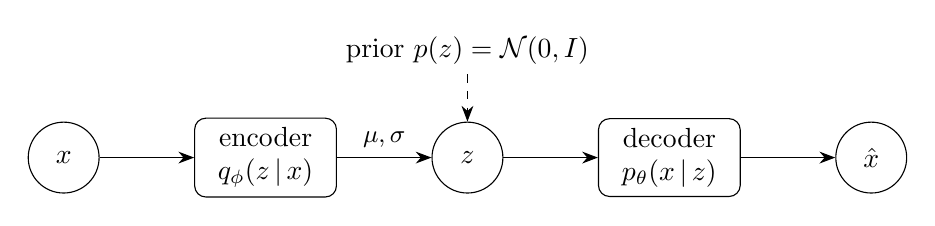
\begin{tikzpicture}[
  node distance=9mm and 12mm,
  box/.style={draw,rounded corners,minimum width=18mm,minimum height=9mm,align=center},
  var/.style={draw,circle,minimum size=9mm},
  >={Stealth[length=2mm]}]
  \node[var] (x) {$x$};
  \node[box,right=of x] (enc) {encoder\\ $q_\phi(z\given x)$};
  \node[var,right=of enc] (z) {$z$};
  \node[box,right=of z] (dec) {decoder\\ $p_\theta(x\given z)$};
  \node[var,right=of dec] (xh) {$\hat x$};
  \node[above=6mm of z] (prior) {prior $p(z)=\mathcal N(0,I)$};
  \draw[->] (x) -- (enc);
  \draw[->] (enc) -- node[above,font=\small]{$\mu,\sigma$} (z);
  \draw[->] (z) -- (dec);
  \draw[->] (dec) -- (xh);
  \draw[->,dashed] (prior) -- (z);
\end{tikzpicture}
\caption{The two networks in a VAE. The encoder maps $x$ to the parameters of a distribution over $z$; the decoder maps a sample $z$ back to a distribution over $x$. The dashed arrow is the sampling path used at generation time: draw $z$ from the prior and decode.}
\end{figure}

\subsection{Autoencoders: useful representations, not a generative model}
A regular (deterministic) autoencoder looks almost identical: an encoder network compresses $x$ into a low-dimensional code $z$, and a decoder reconstructs $x$ from $z$. Training the pair end-to-end with a reconstruction loss (for example, mean squared error) gives a useful representation: the bottleneck $z$ captures the structure the decoder needs in order to rebuild $x$. Foster covers this construction in Chapter 3 of \emph{Generative Deep Learning} (2nd ed., 2023).

\textbf{Why is this not a generative model?} Three concrete problems.
\begin{itemize}[leftmargin=1.2em]
  \item \textbf{No prior on $z$.} The encoder is free to place each training point anywhere in the latent space. If you sample a random $z$ at inference time and decode it, you will probably land in a region the encoder never used; the decoder has no idea what to do, and the output is gibberish.
  \item \textbf{No probability over $x$.} The decoder produces a single reconstruction, not a distribution. You cannot ask ``how likely is this $x$?''
  \item \textbf{Reconstruction-only objective.} Nothing in the loss encourages the latent space to be coherent for sampling.
\end{itemize}
A vanilla autoencoder is therefore a good \emph{representation learner}, but not a \emph{sampler}. The VAE fixes this with three changes: a prior on $z$, probabilistic encoder and decoder, and a regularizer that pulls the encoded distributions toward the prior. Those three changes turn the autoencoder into a generative model.

\subsection{Representation learning, briefly}
Even setting aside generation, latent-variable models are valuable because the latent space is often a much better representation of $x$ for downstream tasks (classification, clustering, similarity search, anomaly detection) than the raw pixels. A good latent space is
\begin{itemize}[leftmargin=1.2em]
  \item \emph{smooth}: nearby $z$ decode to similar $x$;
  \item \emph{structured}: semantic factors of variation correspond to specific directions in $z$;
  \item \emph{low-dimensional}: much smaller than $\dim(x)$ without losing the information you care about.
\end{itemize}
Topic 3 returns to this when we look at latent-space interpolation and arithmetic. See Bengio, Courville, and Vincent, ``Representation Learning: A Review and New Perspectives'' (IEEE TPAMI, 2013; arXiv:1206.5538) for background on what makes a representation good.

\subsection{Payoff}
Everything that follows is a way of making the two operations above (generate, infer) tractable when the decoder is a neural network. Topic 2 handles the intractable marginal and posterior and derives the training objective (the ELBO). Topic 3 turns the ELBO into a concrete loss and shows what sampling looks like. Topic 4 covers the practical knobs you need for the coding assignment.

% ===========================================================================
\section{Topic 2: Variational Inference and the ELBO}
% ===========================================================================

\subsection{Plain-English summary}
We want to fit a generative model that has a hidden variable inside it. The standard way to train such a model is to maximize the likelihood of the data, but for any interesting decoder the likelihood involves an integral we cannot compute. The fix has two moves: (1) introduce an \emph{approximate} answer to ``what hidden state probably produced this data point?'' using a neural network called the \emph{encoder}; and (2) replace the impossible likelihood with the \textbf{Evidence Lower Bound (ELBO)}, which we \emph{can} compute and which is guaranteed to sit at or below the true log-likelihood. Maximizing the ELBO trains the encoder and decoder together with ordinary gradient descent, with one extra trick (reparameterization) to make random sampling differentiable.

\subsection{Overview of this topic}
\begin{itemize}[leftmargin=1.2em]
  \item We begin with the VAE setting: a latent-variable model $p_\theta(x,z)=p(z)\,p_\theta(x\given z)$ and an encoder $q_\phi(z\given x)$ that approximates the intractable posterior.
  \item We derive the ELBO in \textbf{two ways}: (A) via \textbf{Jensen's inequality}; (B) via a \textbf{KL decomposition} that shows the gap to $\log p_\theta(x)$ is $\KL\!\big(q_\phi(z\given x)\,\|\,p_\theta(z\given x)\big)$.
  \item We clarify the \textbf{sign}: $\text{ELBO} = \text{reconstruction} - \KL\!\big(q_\phi(z\given x)\,\|\,p(z)\big)$.
  \item We explain the $\KL(q\,\|\,p)$ notation (the vertical bars are an \emph{ordered-argument separator}, not an absolute value; the order matters because KL is asymmetric).
  \item We show how Eq.\,(2) in Kingma and Welling (2014) becomes their Eq.\,(3) by expanding $\log p_\theta(x,z)$ and recognizing a negative KL term.
\end{itemize}

\subsection{Acronyms and notation}
\begin{description}[style=nextline,leftmargin=1.8em,labelsep=0.6em]
  \item[VAE] \textbf{Variational Autoencoder}: latent-variable model with probabilistic encoder $q_\phi(z\given x)$ and decoder $p_\theta(x\given z)$ trained by maximizing the ELBO.
  \item[ELBO] \textbf{Evidence Lower Bound}: computable lower bound on $\log p_\theta(x)$,
  \[
  \mathcal L(\theta,\phi;x) = \E_{q_\phi(z\given x)}[\log p_\theta(x\given z)] - \KL\!\big(q_\phi(z\given x)\,\|\,p(z)\big).
  \]
  \item[KL] \textbf{Kullback-Leibler divergence}: $\KL(q\,\|\,p)=\int q(z)\log\frac{q(z)}{p(z)}\,dz=\E_q\!\big[\log \tfrac{q}{p}\big]$; asymmetric measure of discrepancy between distributions.
  \item[SGVB] \textbf{Stochastic Gradient Variational Bayes}: reparameterized Monte Carlo estimator of the ELBO enabling backpropagation.
  \item[AEVB] \textbf{Auto-Encoding Variational Bayes}: application of SGVB with neural encoders and decoders (what is now called VAE training).
  \item[i.i.d.] \textbf{Independent and identically distributed}: common assumption for datapoints in a dataset.
  \item[BCE] \textbf{Binary Cross-Entropy}: negative log-likelihood for Bernoulli observation models.
  \item[MSE] \textbf{Mean Squared Error}: corresponds (up to constants) to Gaussian negative log-likelihood with fixed variance.
  \item[PDF/CDF] \textbf{Probability Density Function} and \textbf{Cumulative Distribution Function}.
  \item[RT] \textbf{Reparameterization Trick}: write $z=g_\phi(\varepsilon,x)$ with $\varepsilon$ independent of $\phi$ (e.g., $\varepsilon\sim\mathcal N(0,I)$) so gradients can flow.
  \item[$\odot$] Elementwise (Hadamard) product.
  \item[$\mathcal N(\mu,\Sigma)$] Multivariate normal with mean $\mu$ and covariance $\Sigma$; $\mathcal N(0,I)$ is standard normal.
  \item[$\mathrm{diag}(\sigma^2)$] Diagonal covariance matrix with entries $\sigma_1^2,\dots,\sigma_k^2$.
  \item[$x,z$] Observed data $x$ and latent variable $z$.
  \item[$p_\theta(x\given z)$] Decoder / likelihood; $\theta$ are generative parameters.
  \item[$q_\phi(z\given x)$] Encoder / variational posterior; $\phi$ are recognition parameters.
  \item[$p(z)$] Prior over latents (often $\mathcal N(0,I)$).
  \item[$\mu(x),\sigma(x)$] Encoder outputs parameterizing $q_\phi(z\given x)$ (typically diagonal Gaussian).
  \item[$\varepsilon\sim\mathcal N(0,I)$] Parameter-free noise used in the reparameterization $z=\mu(x)+\sigma(x)\odot\varepsilon$.
\end{description}
Expectations with respect to a density $r$ are written $\E_r[\cdot]$.

\subsection{Prerequisites (quick refresher)}
\subsubsection*{Random variables, densities, expectations}
Let $Z$ be a random variable with density $r(z)$. For any integrable function $f$,
\[
\E_{Z\sim r}[f(Z)] \;=\; \int f(z)\, r(z)\,dz.
\]
We often shorten to $\E_{r}[f(Z)]$ or $\E_r[f(z)]$.

\subsubsection*{Log-likelihoods and nats}
We use natural logarithms. Quantities like $\log p(\cdot)$ are in \emph{nats}. (Base-2 logs would measure in \emph{bits}.)

\subsubsection*{Concavity and Jensen's inequality}
A function $f$ is \emph{concave} if for $0\le \lambda \le 1$,
$f(\lambda a+(1-\lambda)b)\ge \lambda f(a)+(1-\lambda)f(b)$. The $\log(\cdot)$ function is concave. \textbf{Jensen's inequality} says that for a concave $f$ and a random variable $Y$,
\[
f\!\big(\E[Y]\big)\;\ge\;\E[f(Y)] .
\]
In particular, for $f=\log$,
\[
\log \E[Y] \;\ge\; \E[\log Y].
\]
\emph{Plain English:} a concave function like $\log$ ``bends downward,'' so applying $\log$ \emph{after} averaging yields a value \emph{no smaller} than averaging the logged values. This lets us swap a hard ``$\log$ of an expectation'' for an easier ``expectation of a $\log$,'' creating a useful lower bound.

\subsubsection*{Bayes' rule and the posterior}
For a joint density $p_\theta(x,z)=p(z)\,p_\theta(x\given z)$, the posterior is
\[
p_\theta(z\given x) \;=\; \frac{p_\theta(x,z)}{p_\theta(x)} \;=\; \frac{p(z)\,p_\theta(x\given z)}{\int p(z')\,p_\theta(x\given z')\,dz'}.
\]
In many models, this integral (the \emph{evidence}) is intractable.

\subsubsection*{Support / absolute continuity (why it matters)}
To define $\KL(q\,\|\,p)$ and expectations like $\E_q[\log p]$, we require that wherever $q(z)>0$, $p(z)>0$ as well (i.e., $q$ is absolutely continuous w.r.t.\ $p$ on the support of interest). This avoids division-by-zero and $-\infty$ issues.

\subsection{Kullback-Leibler (KL) divergence: definition, notation, intuition}
\subsubsection*{Definition and equivalent forms}
Let $q$ and $p$ be densities on the same support. The KL divergence (from $q$ to $p$) is
\[
\KL(q\,\|\,p) \;=\; \int q(z)\,\log\frac{q(z)}{p(z)}\,dz
\;=\; \E_{q}\!\left[\log\frac{q(z)}{p(z)}\right].
\]

\subsubsection*{Meaning of the vertical bars}
The notation $\KL(q\,\|\,p)$ is read ``KL of $q$ relative to $p$.'' \textbf{The vertical bars ``$\|\,$''} are \emph{just a separator of ordered arguments}. The first argument ($q$) supplies the measure of the expectation. \emph{It is not} an absolute value, a norm, or a conditioning operator. The order matters:
\[
\KL(q\,\|\,p) \neq \KL(p\,\|\,q) \quad\text{in general.}
\]

\subsubsection*{Core properties (why it is a divergence)}
\begin{itemize}[leftmargin=1.2em]
  \item \textbf{Nonnegativity (Gibbs' inequality):} $\KL(q\,\|\,p)\ge 0$, with equality iff $q=p$ almost everywhere.
  \item \textbf{Asymmetry:} $\KL(q\,\|\,p)\neq \KL(p\,\|\,q)$ in general.
  \item \textbf{Link to (cross-)entropy:} $\KL(q\,\|\,p)=H(q,p)-H(q)$, where $H(q)=-\E_q[\log q]$ and $H(q,p)=-\E_q[\log p]$.
  \item \textbf{Coding view (plain English):} $\KL(q\,\|\,p)$ is the \emph{extra code-length} (in nats) you pay on average if data truly come from $q$ but you encode them with a code optimized for $p$.
\end{itemize}
The Gaussian closed form used in VAE code, and a worked example of asymmetry, appear in Topic 3.

\subsection{The VAE setting and objective}
We model data $x$ with latent $z$:
\[
p_\theta(x,z)=p(z)\,p_\theta(x\given z),\qquad p(z)=\mathcal N(0,I)\ \text{(typical)}.
\]
The true posterior $p_\theta(z\given x)$ is often intractable. We introduce a tractable \emph{encoder} $q_\phi(z\given x)$ to approximate it and optimize a lower bound on $\log p_\theta(x)$, the \emph{ELBO}.

\paragraph{Variational inference as optimization.}
The true posterior is the right answer to the question ``given that I observed this $x$, what hidden state $z$ most likely produced it?'' We cannot write it down, so we pick a tractable family $q_\phi(z\given x)$ (in practice a diagonal Gaussian whose mean and standard deviation are produced by a neural network with parameters $\phi$) and look for the member of that family closest to the true posterior in the KL sense:
\[
q_\phi^{\star}(z\given x) \;=\; \argmin_{q_\phi}\; \KL\!\big(q_\phi(z\given x)\,\|\,p_\theta(z\given x)\big).
\]
This is the central trade: an integration problem we cannot solve becomes an optimization problem we can. From here on we learn $\phi$ (encoder) and $\theta$ (decoder) jointly by gradient descent.

\subsection{ELBO derivation A (via Jensen's inequality)}
\subsubsection*{Step-by-step (math)}
\begin{enumerate}[leftmargin=1.6em]
  \item Evidence (marginal likelihood):
  \[
  \log p_\theta(x)=\log \int p_\theta(x,z)\,dz.
  \]
  \item Insert $q_\phi(z\given x)$ (change of measure):
  \[
  \log p_\theta(x)
  = \log \int q_\phi(z\given x)\,\frac{p_\theta(x,z)}{q_\phi(z\given x)}\,dz
  = \log \E_{q_\phi}\!\left[\frac{p_\theta(x,z)}{q_\phi(z\given x)}\right].
  \]
  \item Concavity of $\log$ (Jensen):
  \[
  \log p_\theta(x)\;\ge\; \E_{q_\phi}\!\left[\log p_\theta(x,z)-\log q_\phi(z\given x)\right].
  \]
  \item Expand the joint:
  \[
  \log p_\theta(x,z)=\log p_\theta(x\given z)+\log p(z).
  \]
  \item Collect terms:
  \[
  \boxed{\;
  \mathcal L(\theta,\phi;x)
  = \E_{q_\phi}[\log p_\theta(x\given z)]
  - \KL\!\big(q_\phi(z\given x)\,\|\,p(z)\big)
  \;\le\; \log p_\theta(x)\;}
  \]
\end{enumerate}

\subsubsection*{Step-by-step (plain English)}
\begin{enumerate}[leftmargin=1.6em]
  \item We want $\log p_\theta(x)$ but integrating over $z$ is hard.
  \item Rewrite that integral as an expectation under a distribution we control (the encoder $q_\phi$).
  \item Use the ``$\log$ bends downward'' trick to turn a hard $\log$ of an average into an easier average of a $\log$, producing a lower bound.
  \item Split the joint into likelihood and prior pieces.
  \item The bound is ``\textbf{reconstruction} minus \textbf{regularizer}''; the regularizer keeps $q_\phi(z\given x)$ near $p(z)$.
\end{enumerate}

\paragraph{When is it tight?}
Equality in Jensen holds iff $\frac{p_\theta(x,z)}{q_\phi(z\given x)}$ is (a.s.) constant in $z$, i.e.\ when $q_\phi(z\given x)=p_\theta(z\given x)$.

\subsection{ELBO derivation B (KL decomposition / ``gap'' identity)}
\subsubsection*{Step-by-step (math)}
\begin{enumerate}[leftmargin=1.6em]
  \item Start with a nonnegative divergence:
  \[
  \KL\!\big(q_\phi(z\given x)\,\|\,p_\theta(z\given x)\big)\;\ge\;0.
  \]
  \item Bayes: $p_\theta(z\given x)=\frac{p_\theta(x,z)}{p_\theta(x)}$:
  \[
  \KL
  = \E_{q_\phi}\!\big[\log q_\phi(z\given x)-\log p_\theta(x,z)+\log p_\theta(x)\big].
  \]
  \item Rearranging gives
  \[
  \boxed{\;
  \log p_\theta(x)
  = \underbrace{\E_{q_\phi}\!\big[\log p_\theta(x,z)-\log q_\phi(z\given x)\big]}_{\text{ELBO}}
  + \KL\!\big(q_\phi(z\given x)\,\|\,p_\theta(z\given x)\big)\; }.
  \]
  \item Expanding the joint recovers the same two-term ELBO as in Derivation A.
\end{enumerate}

\subsubsection*{Step-by-step (plain English)}
\begin{enumerate}[leftmargin=1.6em]
  \item KL is never negative, so it can quantify a ``gap to optimality.''
  \item Bayes' rule inserts $\log p_\theta(x)$ as a constant inside the expectation.
  \item Rearrangement shows: $\log p_\theta(x) = \text{ELBO} + \text{gap}$, therefore ELBO is a lower bound.
  \item If $q_\phi$ equals the true posterior, the gap vanishes and the bound is exact.
\end{enumerate}

\paragraph{What the identity buys us.}
The right-hand side has one piece we can compute (the ELBO) and one we cannot (the KL to the true posterior). If we push the ELBO up by changing $\theta$ and $\phi$, the identity forces one of two things to happen: either $\log p_\theta(x)$ goes up (the model fits the data better) or the KL gap shrinks (the approximate posterior gets closer to the true one). Both are good, and both come from the same gradient step.

\subsection{How Eq.\,(2) becomes Eq.\,(3) in Kingma and Welling}
Starting from (their Eq.\,(2))
\[
\mathcal L(\theta,\phi;x)
= \E_{q_\phi(z\given x)}\big[-\log q_\phi(z\given x)+\log p_\theta(x,z)\big],
\]
expand $\log p_\theta(x,z)=\log p_\theta(x\given z)+\log p(z)$ and regroup:
\[
\mathcal L(\theta,\phi;x)
= \E_{q_\phi}\![\log p_\theta(x\given z)]
+ \E_{q_\phi}\![\log p(z)-\log q_\phi(z\given x)]
= \E_{q_\phi}\![\log p_\theta(x\given z)]
- \KL\!\big(q_\phi(z\given x)\,\|\,p(z)\big),
\]
which is their Eq.\,(3).

\paragraph{Plain English.} Replace the joint by likelihood $+$ prior, then recognize the second expectation as a \emph{negative} KL because $\KL(q\,\|\,p)=\E_q[\log q-\log p]$.

\paragraph{Read the result as a tug-of-war.} The first term asks: when the encoder turns $x$ into a distribution over $z$, and the decoder turns a sampled $z$ back into a distribution over $x$, how well do we recover the original $x$? The second term asks: is the distribution the encoder produced for this $x$ close to the prior we will sample from later? The two terms genuinely fight. Reconstruction alone would let the encoder give each training point its own private corner of latent space (great reconstruction, useless for sampling); the KL alone would let the encoder collapse onto the prior and ignore $x$ (great regularization, nothing left for the decoder). Topic 3 makes this concrete.

\subsection{Reparameterization trick (why we can backprop through sampling)}
The ELBO is an expectation over $q_\phi(z\given x)$, which depends on the encoder parameters $\phi$. If we drew $z$ directly, the gradient with respect to $\phi$ would have to pass through a random sampling step, which has no derivative. Suppose instead that $z\sim q_\phi(z\given x)$ can be written as a differentiable transformation of base noise:
\[
z \;=\; g_\phi(\varepsilon,x),\qquad \varepsilon\sim p(\varepsilon).
\]
\textbf{Gaussian case (common in VAEs):}
\[
z \;=\; \mu_\phi(x) + \sigma_\phi(x)\odot \varepsilon,\qquad \varepsilon\sim\mathcal N(0,I).
\]
Then for any $f$,
\[
\E_{q_\phi(z\given x)}[f(z)]
= \E_{\varepsilon\sim p(\varepsilon)}\!\big[f(g_\phi(\varepsilon,x))\big],
\]
and the right-hand side is differentiable w.r.t.\ $\phi$: gradients $\nabla_\phi$ flow through the deterministic map $g_\phi$.

\paragraph{Plain English.} Move randomness outside the network into a fixed noise source; make the rest deterministic so autodiff works end-to-end. Instead of ``sample $z$ from a distribution whose parameters depend on $\phi$,'' we say ``draw a fixed-distribution $\varepsilon$ once, then transform it through learnable knobs.'' Same result statistically, but now it is differentiable.

\subsection{Sign conventions and what to optimize}
The training objective is to \emph{maximize} the ELBO
\[
\mathcal L(\theta,\phi;x)
= \E_{q_\phi}[\log p_\theta(x\given z)]
- \KL\!\big(q_\phi(z\given x)\,\|\,p(z)\big),
\]
or equivalently \emph{minimize} $-\mathcal L$, which is ``reconstruction loss $+$ KL penalty.'' The ``$+$\;KL'' you sometimes see appears in the identity
\[
\log p_\theta(x)=\text{ELBO}+\KL\!\big(q_\phi(z\given x)\,\|\,p_\theta(z\given x)\big),
\]
where the KL is the nonnegative \emph{gap} to the true log evidence, not part of the ELBO.

\subsection{Key takeaways}
\begin{itemize}[leftmargin=1.2em]
  \item ELBO is a computable lower bound on $\log p_\theta(x)$: \quad
  $\displaystyle \mathcal L=\E_{q_\phi}[\log p_\theta(x\given z)] - \KL(q_\phi(z\given x)\,\|\,p(z))$.
  \item Two derivations: \textbf{Jensen} and \textbf{KL-gap identity}. The ``$+$ KL'' you sometimes see is the \emph{gap}, not part of ELBO.
  \item $\KL(q\,\|\,p)$ is an \emph{ordered} divergence; ``$\|\,$'' is just an argument separator.
  \item Reparameterization lets gradients flow through samples: $z=\mu_\phi(x)+\sigma_\phi(x)\odot\varepsilon$.
  \item The \textbf{encoder} implements $q_\phi(z\given x)$; the \textbf{decoder} implements $p_\theta(x\given z)$. Sampling new data is: draw $z\sim\mathcal N(0,I)$, then decode.
\end{itemize}

\noindent\textbf{Pointer to the original source:} D.\,P.\,Kingma and M.\,Welling, \textit{Auto-Encoding Variational Bayes}, ICLR 2014 (arXiv:1312.6114). A tutorial-length treatment is Kingma and Welling, \textit{An Introduction to Variational Autoencoders}, 2019 (arXiv:1906.02691).

% ===========================================================================
\section{Topic 3: Reconstruction Loss, KL Divergence, and Sampling}
% ===========================================================================

\subsection{Plain-English summary}
Topic 2 derived the ELBO as a single mathematical object. To actually \emph{train} a VAE we need to turn it into code: a loss function with two easy-to-compute pieces, a way to sample from the trained model, and a few diagnostics to check that training is healthy. By the end of this topic you should be able to read the loss function in a standard VAE notebook (for example, Foster's Fashion-MNIST VAE) and explain every line.

\subsection{From ELBO to a practical loss}
The training objective (\emph{maximize} ELBO) is equivalent to \emph{minimizing}
\[
\mathcal L_{\text{VAE}}(\theta,\phi;x) \;=\; -\mathcal L(\theta,\phi;x)
= \underbrace{-\E_{q_\phi}[\log p_\theta(x\given z)]}_{\text{reconstruction loss}}
+ \underbrace{\KL\!\big(q_\phi(z\given x)\,\|\,p(z)\big)}_{\text{KL regularizer}} .
\]
Both pieces have tractable expressions for the choices made below. That is the whole reason we set up the math the way we did.

\subsubsection*{The reconstruction term in practice}
The expectation $\E_{q_\phi(z\given x)}[\log p_\theta(x\given z)]$ is approximated by drawing a single sample $z=\mu_\phi(x)+\sigma_\phi(x)\odot\varepsilon$ (the reparameterization trick) and evaluating $\log p_\theta(x\given z)$ on that sample. One sample per datapoint is enough in practice because we average over a minibatch.

\textbf{Likelihood choices and the corresponding reconstruction term:}
\begin{itemize}[leftmargin=1.2em]
  \item \emph{Bernoulli decoder} (binary or $[0,1]$-valued $x$): $-\E_{q_\phi}[\log p_\theta(x\given z)]$ is the expected \textbf{binary cross-entropy} (BCE), summed over pixels. This is the form used for binarized image data such as Fashion-MNIST.
  \item \emph{Gaussian decoder} (real $x$ with fixed variance $\sigma^2$): $-\E_{q_\phi}[\log p_\theta(x\given z)]$ is (up to constants) proportional to an expected \textbf{mean-squared error} (MSE). This is what most photographic-image VAEs use.
\end{itemize}
The decoder architecture is the same in both cases; only the final activation (sigmoid vs.\ linear) and the loss change.

\subsection{The KL term in closed form}
\subsubsection*{Gaussian closed form (used in VAEs)}
If $q_\phi(z\given x)=\mathcal N(\mu,\mathrm{diag}(\sigma^2))$ in $\R^k$ and $p(z)=\mathcal N(0,I)$,
\[
\KL\!\big(q_\phi(z\given x)\,\|\,p(z)\big) \;=\; \tfrac12 \sum_{i=1}^k\Big(\mu_i^2+\sigma_i^2-\log\sigma_i^2-1\Big).
\]
\emph{Plain English:} penalizes means far from 0 and variances that are too large \emph{or} too small, keeping posteriors smooth and near the prior. This is a single line of code per datapoint. Note that the formula is what fixes the prior to $\mathcal N(0,I)$ in most implementations; swapping the prior requires a different (and usually less convenient) KL expression.

\subsubsection*{Mini example: KL asymmetry with 1D Gaussians}
Let $q=\mathcal N(\mu_q,\sigma_q^2)$, $p=\mathcal N(\mu_p,\sigma_p^2)$. Then
\[
\KL(q\,\|\,p) \;=\; \frac{1}{2}\!\left[\frac{\sigma_q^2}{\sigma_p^2}
+ \frac{(\mu_p-\mu_q)^2}{\sigma_p^2}
-1 + \log\frac{\sigma_p^2}{\sigma_q^2}\right],
\quad
\KL(p\,\|\,q) \;\text{ swaps $(\mu_q,\sigma_q^2)$ and $(\mu_p,\sigma_p^2)$}.
\]
Unless $\mu_q=\mu_p$ and $\sigma_q^2=\sigma_p^2$, the two numbers differ, illustrating \textbf{asymmetry}. Setting $\mu_p=0$, $\sigma_p^2=1$ recovers one term of the VAE closed form above.

\subsection{The reconstruction-vs-regularization tug-of-war, made concrete}
In code you literally watch two scalars compete during training.
\begin{itemize}[leftmargin=1.2em]
  \item \textbf{Reconstruction low, KL high.} The encoder is putting each $x$ far from the prior to give the decoder more capacity. Reconstructions look great; prior samples look terrible.
  \item \textbf{KL near zero, reconstruction high.} The encoder has collapsed $q_\phi(z\given x)$ onto the prior and is ignoring $x$. This is \textbf{posterior collapse}. The prior is well matched; reconstructions are blurry blobs.
\end{itemize}

\subsubsection*{Practical tips and common pitfalls}
\begin{itemize}[leftmargin=1.2em]
  \item \textbf{$\beta$-VAE} (Higgins et al., ICLR 2017): replace the KL term by $\beta\cdot \KL(\cdot)$,
  \[
  \mathcal L_{\beta}(\theta,\phi;x) \;=\; -\E_{q_\phi}[\log p_\theta(x\given z)] + \beta\,\KL\!\big(q_\phi(z\given x)\,\|\,p(z)\big),
  \]
  to enforce disentanglement ($\beta>1$) or boost reconstruction ($\beta<1$). Standard VAE code implicitly uses $\beta=1$; changing it is one line.
  \item \textbf{KL annealing / warm-up}: gradually increase the KL weight from 0 to 1 over the first few epochs to avoid \textit{posterior collapse} (encoder ignored by a strong decoder). Bowman et al., ``Generating Sentences from a Continuous Space'' (CoNLL 2016; arXiv:1511.06349) is the classic worked example in a text-VAE setting.
  \item \textbf{Aggregated posterior vs.\ prior}: even if each $q_\phi(z\given x)$ is close to $p(z)$, the mixture $q(z)=\int q_\phi(z\given x)p_{\text{data}}(x)\,dx$ can deviate; richer priors (e.g., VampPrior, flows) can help.
  \item \textbf{Units}: logs in natural base $\Rightarrow$ losses in \emph{nats}. Switching bases scales constants but not optima.
\end{itemize}

\subsection{Sampling: how a trained VAE generates new data}
Once training is done, generation is two lines:
\begin{enumerate}[leftmargin=1.6em]
  \item Draw $z\sim\mathcal N(0,I)$ from the prior.
  \item Decode: produce $\hat x$ from $p_\theta(x\given z)$. For a Bernoulli decoder the per-pixel probability is your image; for a Gaussian decoder the mean is your image.
\end{enumerate}
That this works at all is the payoff for the KL regularizer: it forces the encoder to use latent positions that are also plausible under the prior, so sampling from the prior lands in regions the decoder knows what to do with. Without the KL term (a vanilla autoencoder), step 2 would produce gibberish.

\subsection{Latent-space structure: interpolation and arithmetic}
A well-trained VAE has a latent space that is smooth and semantically organized. Two visualizations, both easy to reproduce on Fashion-MNIST or a face dataset:
\begin{itemize}[leftmargin=1.2em]
  \item \textbf{Linear interpolation.} Pick two real images $x_1,x_2$; encode to get $z_1,z_2$ (use the means $\mu_\phi$). Walk along
  \[
  z(t) = (1-t)\,z_1 + t\,z_2,\qquad t\in[0,1],
  \]
  and decode at each step. A trained VAE produces a smooth morph, not a sequence of glitches, because nearby $z$ decode to similar $x$.
  \item \textbf{Latent arithmetic.} Average the latent codes of all training points with attribute A (for example, ``smiling'') and subtract the average code of all points without it. The resulting vector behaves like a direction for that attribute: add it to any encoded $z$ and the decoded image gains the attribute. Foster demonstrates this in Chapter 3.
\end{itemize}

\subsection{Payoff}
The ELBO gives us a loss with two named, computable terms; the closed-form KL and the reparameterized reconstruction make it a few lines of code; and the KL regularizer is exactly what makes ``sample from the prior and decode'' produce sensible outputs. When training misbehaves, the two loss scalars tell you which side of the tug-of-war is winning, and $\beta$ or KL warm-up let you rebalance it.

% ===========================================================================
\section{Topic 4: Practical Considerations When Training and Evaluating a VAE}
% ===========================================================================

\subsection{Plain-English summary}
Topics 1 through 3 told you what a VAE is and what it optimizes. This topic is the ``before you open the notebook'' reference: the architecture choices you will face, the training knobs that actually matter, the failure modes to recognize, the evaluation evidence to trust, and the compute footprint of the assignment.

\subsection{Architecture choices}
The encoder and decoder are independent design problems, but they share a few rules of thumb.
\begin{itemize}[leftmargin=1.2em]
  \item \textbf{Latent dimension $d$.} The single most important hyperparameter. Too small and the decoder cannot reconstruct meaningful detail; too large and the KL regularizer has trouble keeping the posterior compact. Common starting points: $d=2$ for visualization, $d=10$ to $50$ for Fashion-MNIST, $d=100$ to $200$ for face datasets.
  \item \textbf{Encoder network.} For images, a few convolutional layers with stride-2 downsampling, ending in two parallel fully-connected heads that output $\mu_\phi(x)$ and $\log\sigma^2_\phi(x)$. Outputting the \emph{log}-variance keeps the value unconstrained and numerically stable:
  \[
  \sigma_\phi(x) = \exp\!\big(\tfrac12 \log\sigma^2_\phi(x)\big), \qquad z=\mu_\phi(x)+\sigma_\phi(x)\odot\varepsilon .
  \]
  \item \textbf{Decoder network.} Mirror image of the encoder: fully-connected to a small spatial volume, then transposed convolutions (or upsampling plus regular convolutions) up to the input resolution. Final activation is sigmoid for $[0,1]$ pixel data (Bernoulli decoder) or linear for general-range data (Gaussian decoder).
  \item \textbf{Symmetry.} Encoder and decoder do not strictly need to be symmetric, but starting symmetric is a sensible default.
\end{itemize}

\subsection{Training knobs that matter}
\begin{itemize}[leftmargin=1.2em]
  \item \textbf{Optimizer:} Adam with learning rate around $10^{-3}$ or $5\cdot 10^{-4}$. Almost never the bottleneck.
  \item \textbf{Batch size:} 64 to 256 is fine for Fashion-MNIST on a laptop. Larger batches give more stable KL estimates but cost memory.
  \item \textbf{KL warm-up:} ramp the KL coefficient from 0 to 1 over the first 5 to 20 epochs. Helps avoid posterior collapse, especially when $d$ is large.
  \item \textbf{Number of epochs:} 20 to 50 for Fashion-MNIST is usually enough to see a clear pattern; longer is rarely transformative.
  \item \textbf{Reproducibility:} set a fixed random seed for NumPy, the framework (TensorFlow or PyTorch), and the dataloader. Log the seed in your write-up.
\end{itemize}

\subsection{Failure modes to recognize}
\begin{itemize}[leftmargin=1.2em]
  \item \textbf{Posterior collapse.} KL loss collapses to (near) zero early in training. Symptom: the encoder ignores $x$, so reconstructions look like a single average image regardless of input. Remedies: KL warm-up, smaller $\beta$, more capacity in the decoder bottleneck.
  \item \textbf{Blurry reconstructions.} The classic VAE failure mode. Most often a consequence of the Gaussian decoder assumption (the mean of a multimodal distribution \emph{is} blurry). Often acceptable; not the same problem as posterior collapse.
  \item \textbf{Exploding variance.} If $\log\sigma^2_\phi$ is not bounded, training can drift into unreasonably large variances. Clipping the log-variance to, say, $[-5,5]$ is a simple guard.
  \item \textbf{Mode dropping.} Samples cover only some of the modes of the data distribution. Less common in VAEs than in GANs, but watch for it in your prior-sample grids.
\end{itemize}

\subsection{Evaluation: how do you know it worked?}
VAE evaluation is genuinely hard, because no single number captures ``sample quality.'' Combine three kinds of evidence.
\begin{enumerate}[leftmargin=1.6em]
  \item \textbf{Loss curves.} Plot total loss, reconstruction loss, and KL loss separately as a function of epoch. Both terms should decrease at first; KL typically rises slightly later as the model trades off. Big gaps or single-term collapses are red flags.
  \item \textbf{Sample quality.} Draw a grid (e.g., 16 samples) from the prior and decode. Inspect by eye. For Fashion-MNIST you should recognize garment classes after a few epochs.
  \item \textbf{Latent-space structure.} Encode the test set, take the means $\mu_\phi(x)$, and either scatter directly (if $d=2$) or project with t-SNE or UMAP. Color points by class label. A well-trained VAE shows class clusters even though it was trained without labels.
\end{enumerate}
Quantitative metrics such as FID (Fr\'echet Inception Distance) and IS (Inception Score) exist but are most useful for comparing methods on the same benchmark; they are overkill for the Module 2 assignment.

\subsection{Compute footprint}
The Fashion-MNIST VAE notebook trains in roughly 5 to 15 minutes on a CPU laptop. You do not need a GPU for the required assignment. If your machine struggles, the university HPC cluster via Open OnDemand JupyterLab (covered in Module 1) is the recommended fallback. The stretch face-dataset notebook benefits noticeably from a GPU.

\subsection{Payoff}
You are now ready for the Module 2 VAE Technical Assignment: run the Fashion-MNIST VAE, vary the latent dimension, sample from the prior, visualize the latent space, and write a short interpretation. Topic 3 gave you the loss-function vocabulary; this topic gave you the diagnostics and the architecture defaults. If you can read the two loss scalars, look at a prior-sample grid, and look at a class-colored latent scatter, you can diagnose most of what goes wrong with a VAE.

\subsection*{References and further reading}
\begin{itemize}[leftmargin=1.2em]
  \item D. P. Kingma and M. Welling, ``Auto-Encoding Variational Bayes,'' ICLR 2014. arXiv:1312.6114.
  \item D. P. Kingma and M. Welling, \emph{An Introduction to Variational Autoencoders}, 2019. arXiv:1906.02691.
  \item C. Doersch, ``Tutorial on Variational Autoencoders,'' 2016. arXiv:1606.05908.
  \item I. Higgins et al., ``$\beta$-VAE: Learning Basic Visual Concepts with a Constrained Variational Framework,'' ICLR 2017.
  \item S. R. Bowman et al., ``Generating Sentences from a Continuous Space,'' CoNLL 2016. arXiv:1511.06349.
  \item D. Rezende and S. Mohamed, ``Variational Inference with Normalizing Flows,'' ICML 2015. arXiv:1505.05770.
  \item D. Kingma et al., ``Improved Variational Inference with Inverse Autoregressive Flow,'' NeurIPS 2016. arXiv:1606.04934.
  \item Y. Bengio, A. Courville, and P. Vincent, ``Representation Learning: A Review and New Perspectives,'' IEEE TPAMI, 2013. arXiv:1206.5538.
  \item I. Goodfellow, Y. Bengio, and A. Courville, \emph{Deep Learning}, MIT Press, 2016, Chapter 14 (Autoencoders).
  \item D. Foster, \emph{Generative Deep Learning}, 2nd ed., O'Reilly, 2023, Chapter 3 (Variational Autoencoders). Companion notebooks: \url{https://github.com/davidADSP/Generative_Deep_Learning_2nd_Edition}.
\end{itemize}

\end{document}
